\section{Brownian motion}
Brownian motion is the motion that occurs when looking at microscopic particles that are suspended in a fluid, this motion is highly random and is due to molecules in the fluid colliding with the particle trillions of times per second. In principle if one knew the momenta and positions of all particles in a system, then one could use Newtonian mechanics to fully predict the future state of the system. However, for systems of interest in this project, we will be looking at systems with particle number on the order of Avagadro's number ($N \sim 10^{23}$). With systems of this size, a Newtonian description is completely impractical, so instead we will use a statistical approach, in this view the motion of a single Brownian particle suspended in a fluid at a given temperature (which we will call the bath) is random.

Brownian motion was first observed by Robert Brown in 1827 \cite{Brown1828}, in these observations, Brown saw that microscopic particles (for example pollen grains) were in constant motion. He noticed that this motion was still present in inorganic material including granite and ground up Sphinx bones.
\begin{quote}
To mention all the mineral substances in which I have found these molecules, would be tedious; and I shall confine myself in this summary to an enumeration of a few of the most remarkable. These were both of aqueous and igneous origin, as travertine, stalactites, lava, obsidian, pumice, volcanic ashes, and meteorites from various localities. Of metals I may mention manganese, nickel, plumhago, bismuth, antimony, and arsenic. In a word, in every mineral which I could reduce to a powder, sufficiently fine to be temporarily suspended in water, I found these molecules more or less copiously; and in some cases, more particularly in siliceous crystals, the whole body submitted to examination appeared to be composed of them. --\textbf{Robert Brown on what we now call Brownian particles}
\end{quote}
Over half a century later, Einstein showed that Brownian motion was due to constant bombardment by water molecules in the surrounding environment \cite{Einstein1905}, Einsteins theory of Brownian motion was then experimentally verified by Perrin \cite{Perrin2013}. The trajectory of a single Brownian particle can either be described stochastically or an ensemble of Brownian particles can be described by a probability distribution. Work at around the same time by Smoluchowski allows us to determine the evolution of the probability distribution of a Brownian particle mathematically using the Smoluchowksi equation which we will discuss in ~\autoref{Smoluchowski}. We will think of a Brownian particle moving in titled periodic potential of the form $V(x)$, as shown schematically in figure \ref{fig:Schematic}. In this figure we have a particle with a certain known probability density, the particle is agitated by thermal vibrations in a random diffusive manner, however there is also a forcing on the particles that we describe using the potential.

\section{Brownian motors}
Brownian motors are devices that can use stored chemical energy to create directed motion on a microscopic scale, they are ubiquitous in biology where they are used to perform important tasks in cells  \cite{PhillipsQuakeMay2006, Magnasco1994} this is done by transforming energy from one degree of freedom to another. Recently, thanks to improvements in imaging techniques, researchers have been able to make highly detailed images of these motors and their working components \cite{YiWeiChang2016}. As well as being able to crank a rotor in the in the fashion of a traditional motor, Brownian motors are also able to pump ions against a gradient and translocate molecules\cite{Magnasco1994, Reimann2001, Leibler1993, leibler1990physical}. Brownian motors have also been investigated in the laboratory, for example Ref \cite{BlickleBechinger2011} created a stochastic heat engine by placing a single colloidal particle in a time dependent optical trap. Likewise, Ref \cite{Pedro2014} placed a colloidal particle in an optical tweezer and drove the particle with explosive vaporization of the surrounding liquid, thus demonstrating a thermal mechanism for Brownian motors. Ref \cite{JoelBader1999} placed DNA molecules in a time dependent potential to transport the molecules. Brownian ratchets capable of walking along a track have been implemented in the laboratory recently \cite{Wang2010,DeliusGeertsemaLeigh2010,DeliusGeertsemaLeighEtAl2010}, in order to improve on these designs and to approach the efficiency present in nature, we will have to understand the physics of Brownian dynamics very clearly.

The name Brownian motors is not a misnomer, a Brownian motor can be modeled as a Brownian particle diffusing over its free energy landscape \cite{Reimann2001}, in the case of Brownian motion it is natural to think of the particle moving in a spatial coordinate $x$, however in the case of Brownian motors the interpretation of the coordinate $x$ is more abstract. In general $x$ will be a degree of freedom for the system, examples include reaction coordinates for a chemical reactions, or in the case of a rotary motors, the angle of the motor itself.

\begin{figure}[tb]
	\begin{subfigure}{0.49\textwidth}
		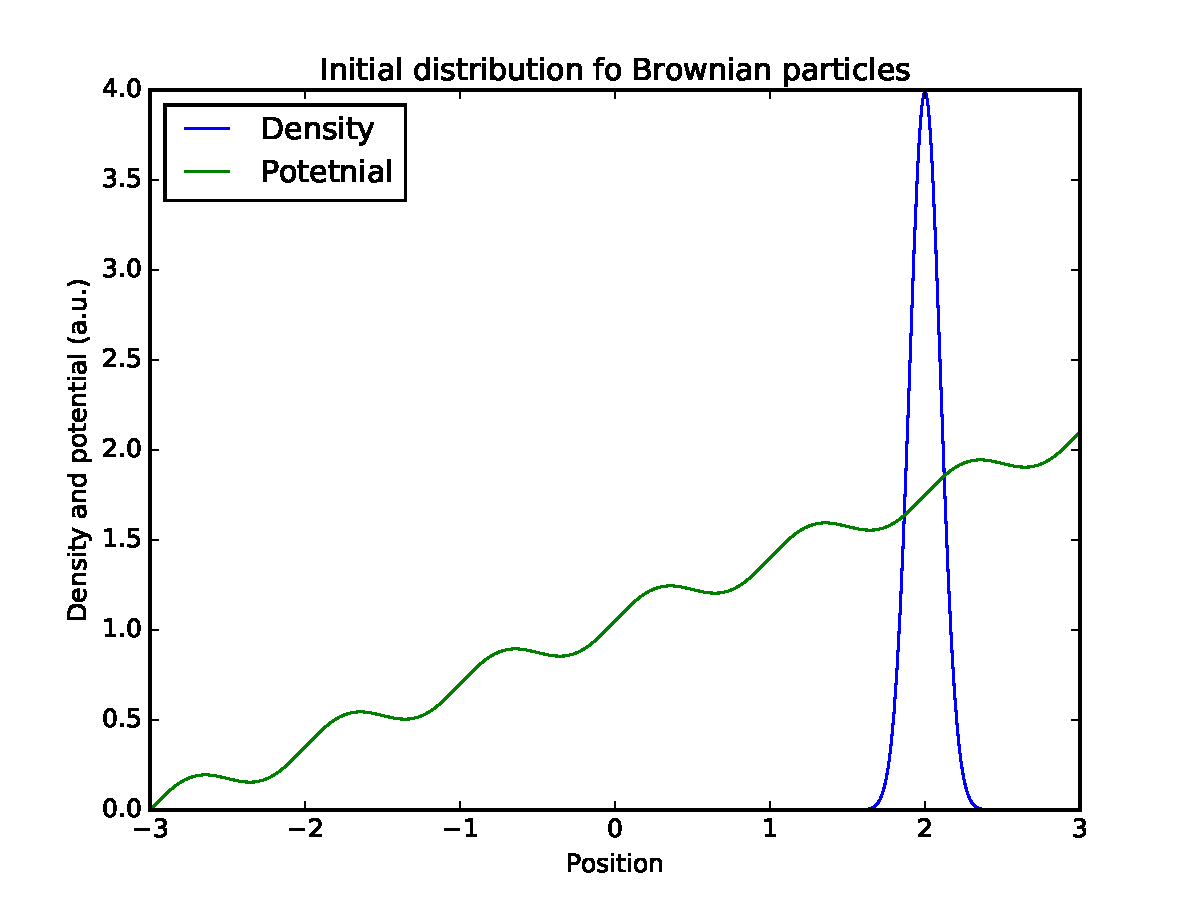
\includegraphics[width=\columnwidth]{SchematicConstantTempInit}
		\caption{\label{fig:Init}}
	\end{subfigure}
\begin{subfigure}{0.49\textwidth}
		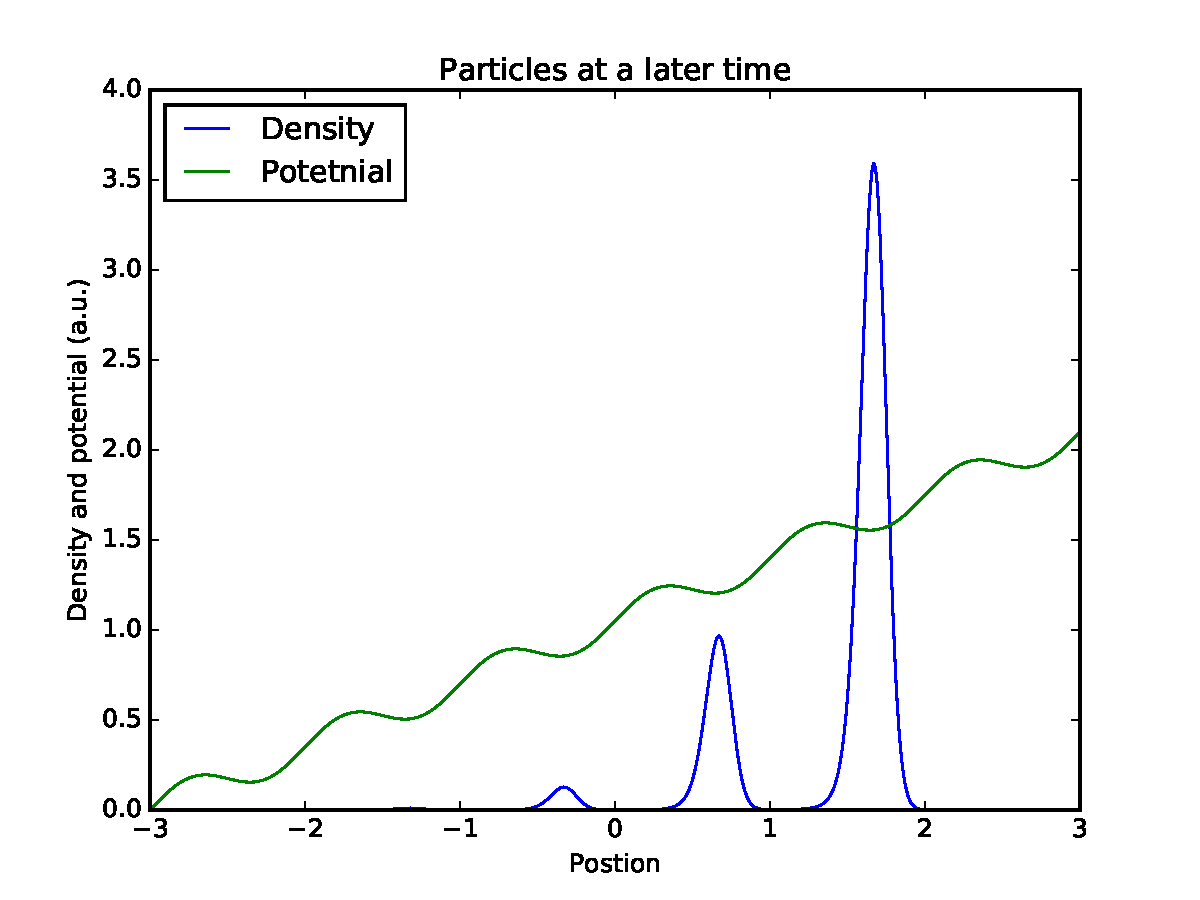
\includegraphics[width=\columnwidth]{SchematicConstantTempFinal}
		\caption{\label{fig:Final}}
\end{subfigure}
\caption{Schematic showing the probability density of particles diffusing in a one dimensional tilted periodic potential at a fixed temperature. We see that the particles tend to drift down the potential as they diffuse, this drift will be called the current $J$ which we will quantify in section ~\autoref{Smoluchowski}.}
\label{fig:Schematic}
\end{figure}

\section{Classes of Brownian motors} \label{BrownianMotorClasses}
Here we will discuss different classes of Brownian motors and their relationship to this project. Different types of Brownian motors have been explored in the literature, including the Feynman ratchet \cite{Feynman1963}, the Landauer blowtorch \cite{Landauer1988}, thermal ratchets \cite{Pedro2014}, time dependent potentials \cite{JoelBader1999,BlickleBechinger2011} and tilted periodic potentials \cite{Leibler1993,Magnasco1994}.

\subsection{Feynman ratchet and pawl {\color{red} fix this section up}}
The Feynman ratchet was initially discussed in the Feynman lectures \cite{Feynman1963} and was at first thought to be able to achieve greater than Carnot efficiency, however closer analysis showed that this was not possible \cite{ParrondoEspanol1996}. The system works as follows, we have two boxes that are thermally insulated from one another that are connected by an axle that can rotate. In one box there is a ratchet and pawl connected to the axle that makes it easy for the axle to turn one way (say clockwise), but hard to turn the other way (anti-clockwise). In the other box the axle is connected to paddles that are being buffeted by a gas (which we call the bath). The motion of the paddles are random since they are dictated by Brownian motion, so the purpose of the ratchet and pawl is to rectify the Brownian motion of these paddles. One may think that this could be used to do work (for example by using the axle to lift a weight), however this is not true. The problem is that the ratchet and pawl themselves will also be subject to random motion so they will sometimes allow the axle to turn anti-clockwise. To model the Feynman ratchet, we will need two degrees of freedom \cite{M.W.Jack2016}, this is beyond the scope of this project because we will only simulate systems with one degree of freedom.

\subsection{Landauer's blowtorch {\color{red} expand}}
\begin{figure}[tb]
	\begin{subfigure}{0.42\textwidth}
		\includegraphics[width=\columnwidth]{landauersBlowtorchA}
		\caption{\label{fig:landauerA}}
	\end{subfigure}
	\begin{subfigure}{0.42\textwidth}
		\includegraphics[width=\columnwidth]{landauersBlowtorchB}
		\caption{\label{fig:landauerB}}
	\end{subfigure}
	\begin{subfigure}{0.12\textwidth}
		\includegraphics[width=\columnwidth]{landauersBlowtorchLegend}
	\end{subfigure}

\caption{Landauers blowtorch in a bi-stable potential: In (a) we see that if the particles are left for a long enough time, then they will reach an equilibrium where the population in the upper well is greater than that in the lower well. In (b) we see that if the temperature in the upper well is lower than that of the lower well, then the euilibrium concentrations can be drastically altered.}
\label{fig:landauersBlowtorch}
\end{figure}
The Landauer blowtorch scheme involves a temperature that varies in space \cite{Landauer1988}. The principle is shown schematically in Figure \ref{fig:landauersBlowtorch}, in this figure the temperature is held fixed by an external heat source and can be made to vary along the potential. The steady state probability distribution was calculated using techniques that are described in ~\autoref{SteadyState}, in reference to this phenomena Landauer says that \cite{Landauer1988} ``The relative occupation of competing states of local stability is not determined solely by the characteristics of the locally favored states, but depends on the noise along the whole path connecting the competing states." The reason that particles move against the potential gradient is that where the potential is heated, the particles become more agitated, therefore we should expect that the probability of finding a particle in a hot region is small. A common analogy due to G. E. Hinton is pebbles on a driveway, if one places pebbles on a driveway in a uniform fashion, then after some time one will find that the pebbles will pile up on the side of the driveway where there is no traffic. This occurs despite the fact that the car exerts no nett sideways force on the pebbles, the explanation of this phenomena is that the car is agitating the pebbles in the center effectively at random, but once the pebbles leave the center they experience no agitation (zero temperature) and so they will stay in place. This has caused some authors to describe the temperature as an effective potential \cite{Gardiner2009, Kampen1988}, in particular \cite{DasDasBarikEtAl2015} report a so called reverse Landauer blowtorch effect. In this paper, the authors report show that if one begins with particles in the upper well of a bi-stable potential, then as the particles move to the lower well, they will reduce the temperature of the upper well. In section ~\autoref{Kramers}, we will discuss the reverse Landauer blowtorch and it's effect on the Kramer's rate in more detail.

\subsection{Tilted periodic potentials}
The tilted periodic potential (Figure \ref{fig:Schematic}) is of particular interest for this project because it can be used to model biological motors \cite{Leibler1993,Magnasco1994}. In this model, the potential can be a very complicated function of space despite the fact that temperature is held fixed. One way to model Brownian motors of this class is to think of a reaction coordinate $x$ that describes the conformation of a molecule in a chemical reaction. An example of this is the reaction ATP $\rightleftharpoons$ ADP + P, where ATP is adenosine tri-phosphate, ADP is adenosine di-phosphate and P is a lone phosphate molecule. This reaction coordinate is then coupled to a mechanical coordinate $y$ so that each time that a reaction takes place, the motor will move in some way. Since this is a chemical reaction, the free energy will be decreased as time moves forwards. So a system that has a potential that is periodic in $x$ is not sufficient to describe this situation, we will need to ``tilt" the potential by adding a forcing $f$. The value of $f$ will depend on the $\Delta G$ of the reaction (i.e. how far out of equilibrium the reaction is). It is shown in \cite{Magnasco1994} that this can be modeled by the two dimensional Smoluchowski equation. In this project we will only be modeling the one dimensional Somluchowski equation, so we will have to consider the case where $x$ and $y$ are tightly coupled. An example of tight coupling is the kinesin motor \cite{Leibler1993} that is used in cells to transport molecules. The kinesin motor is strongly bound to a track that it ``walks" along, on each step the motor will hydrolyze an ATP molecule using the reaction shown above. This reaction liberates about $12 k_B T$ Joules of energy that the motor uses to move forward. Kinesin motors are able to take many steps forward while taking few steps backwards all while falling off their track very infrequently \cite{BlockSM1990}.
